%\section{Selection Cuts for eleTau Channel}
\section{\texorpdfstring{Selection cuts for \leptonTau channel}{Selection cuts for lepton-tau channel}}
\label{sect:eleTauCuts}
In the \leptonTau final states, namely e\Tau and $\mu\Tau$,
two set of combined triggers are used. For the e\Tau channel, a loosely isolated \Tau is requested with \PT $>$ 20 \GeV and $|\eta|$ $<$ 2.3 
accompanied by an isolated electron with $|\eta|$ $<$ 2.1. The minimum \PT of the electron was changed from  20 to  22 \GeV 
during the run to compensate the increase of the instant luminosity.
The $\mu\Tau$ channel has a similar trigger where the \Tau leg is exactly same as the e\Tau channel, but the  isolated $\mu$  
has $|\eta|$ $<$ 2.1 and \PT $>$  17 or 18 \GeV in different periods. 
In the analysis, events are selected when one electron(muon) with \PT $>$ 25 (20) \GeV and $|\eta|$ $<$ 2.1 and at least 
one oppositely charged \Tau with \PT $>$ 20 \GeV and $|\eta|$ $<$ 2.3 exist. %The $I_{\Tau}$ of the hadronic tau must be less than 0.8 \GeV.
The selected objects are required to pass the corresponding tight isolation.
In the case of more than one pair, the pair that maximizes the sum $\PT^{\Tau} + \PT^{\ell}$ is selected.
Vetoing the second lepton with \PT $>$ 10 \GeV and loose isolation criteria helps to suppress the $ZX$ backgrounds.

After requesting two opposite sign leptons in the events, a loose cut on \MET $>$ 30 \GeV is applied to suppress QCD multijet events. 
As there is no b-quark in the signal, rejecting events with one or more b-tagged jets reduces significantly \ttbar and $Wb$ backgrounds.

To reject low mass QCD resonances, the invariant mass of the \leptonTau system  is requested to be greater than 15 \GeV. 
Another cut on the invariant mass is applied to remove the peak of the $\Z$jets events. 
It has been found that the visible mass of the $Z\to\tau\tau\to\,e/\mu +\Tau$ moves to 60 $\pm$ 15 \GeV due to 
mis-reconstruction of the energy of the hadronic $\tau$ and also the missing energy due to the decay of the $\tau$ to leptons. 
So the events with the invariant mass of \leptonTau in the window of [45, 75] are excluded from the analysis (\Z veto). 
The minimum angle in the transverse plane between the \MET and the jets %with \PT $>$ 40 \GeV and $|\eta| <$ 5 
is asked to be greater than 1. This cut and a soft cut on \mttwo ($>$ 40 \GeV) suppresses the bulk of the QCD events. The former cut is useful 
against the $W$jets also.
%to get rid of related uncertainties due to mis-reconstruction of the QCD events. 
%As it has mentioned above, the signal events are expected to have high $MT2$ values due to the intrinsic \MET.
%The cut flow tables for the electron/$\mu$ $\,+\tau$ pre-selections are shown in tables .... and ... respectively. The distribution of the $p_{T}$ of the $\tau$ and $MET$ in the pre-selected events in both channels are shown in FIGS ... . The good agreement between data and MC confirms that the needed correction factors are considered carefully.

Similar to the \tauTau channel, a hard cut on \mttwo ($>$ 90 \GeV) is useful to suppress different SM backgrounds, especially $W$jets events.
Such a high cut on the \mttwo increases the sensitivity of the study to signal events with high mass difference. The \Tau transverse mass (\tauMT)
is found to be a good discriminator to further suppress the $W$jets events which is the main background in this step. 
Opposite to the \tauTau channel, the events with \mttwo $<$ 90 \GeV are not useful in \leptonTau channels and they can not add any power to 
the final exclusion. The signal regions for $e\Tau$ and $\mu\Tau$ channels are defined by the following selections:
\begin{itemize}
\item \mttwo $>$ 90 \GeV.
\item \tauMT $>$ 200 \GeV; 
\end{itemize}

% The composition of the backgrounds and number of remaining signals for both channels can be found in the table \ref{tbl:yieldsLepTau}.

%\begin{table}[!Hhtb]
%\begin{center}
%\begin{tiny}
%\begin{tabular}{lcccccccc}
%\hline
%\hline
%  & SUSY(380,1) & QCD & W & ZX & Top & WW & Higgs & MC \\%& Data \\
%\hline
%\hline
%e\Tau       & 2.14 & 0.0 & 1.29 & 0.38 & 0.02 & 0.05 & 0.06 & 1.79$\pm$0.63 \\%& 3 \\
%\hline
%$\mu\hadtau$& 2.09 & 0.0 & 0.79 & 0.28 & 0.0  & 0.34 & 0.05 & 1.46$\pm$.49 \\%& 5 \\
%QCD 70.87 +- 34.49
%Top 1.15 +- 0.84
%\hline
%\hline
%\end{tabular}
%\caption{MC driven yields for e\Tau and $\mu\hadtau$ channels. Only statistical uncertainties are reported.}
%\label{tbl:yieldsLepTau}
%\end{tiny}
%\end{center}
%\end{table}

Figures \ref{fig:mt2leptontau} and \ref{fig:taumtleptontau} show the \mttwo distribution after preselection cuts and  \tauMT 
distribution after applying the preselection and \mttwo cut, respectively.
\begin{figure}[!Hhtb]
\centering
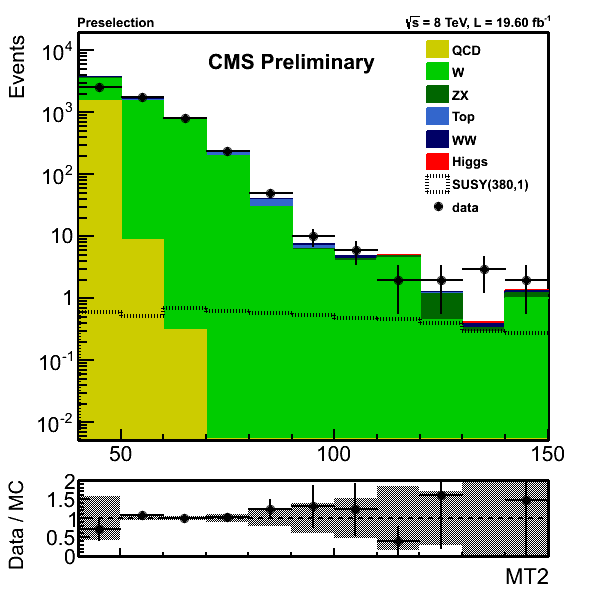
\includegraphics[angle=0,scale=0.35]{SelectionEleTau/MT2.png}
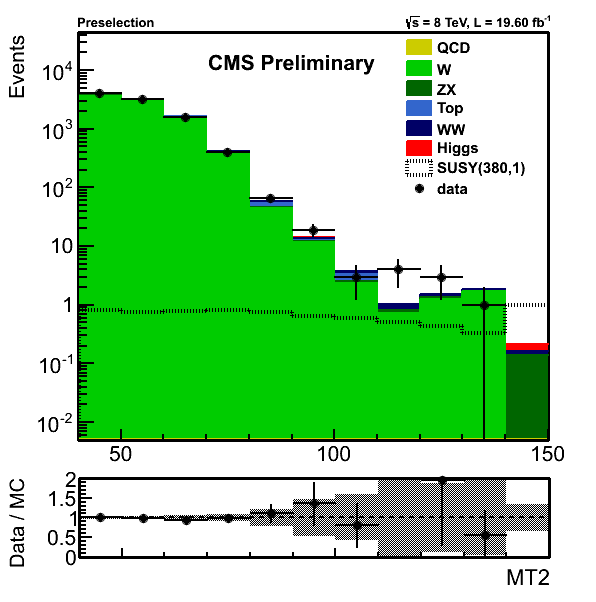
\includegraphics[angle=0,scale=0.35]{SelectionMuTau/MT2_Ratio_Preselection_unBlinded.png}
\caption{\mttwo distribution of preselected events in (left) $e\hadtau$ and (right) $\mu\hadtau$ channels.}
\label{fig:mt2leptontau}
\end{figure}


\begin{figure}[!Hhtb]
\centering
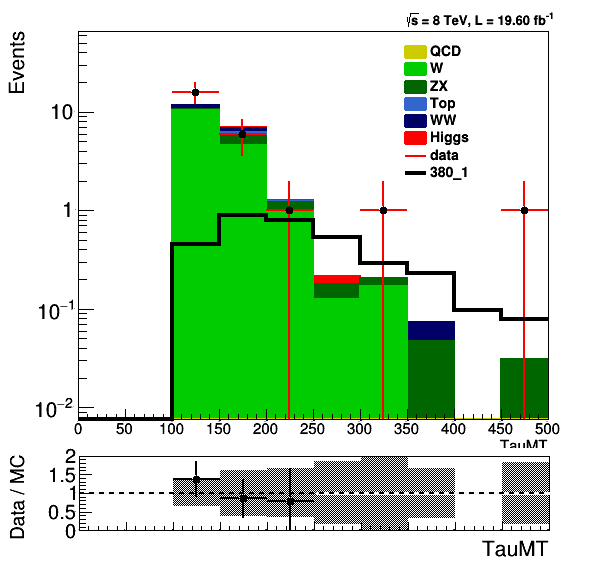
\includegraphics[angle=0,scale=0.35]{SelectionEleTau/TauMT.png}
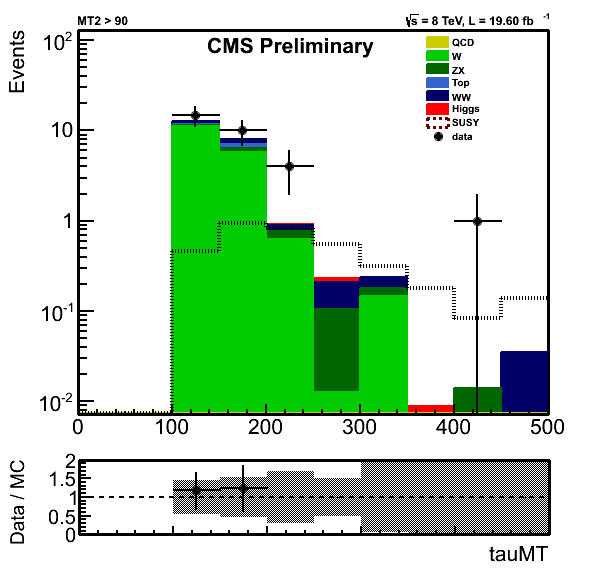
\includegraphics[angle=0,scale=0.35]{SelectionMuTau/tauMT_Ratio_MT2gt90_unBlinded.png}
\caption{\tauMT distribution for events with $\mttwo>$90\GeV in (left) $e\hadtau$ and (right) $\mu\hadtau$ channels.}
\label{fig:taumtleptontau}
\end{figure}
%Opposite to the $\Tau\Tau$ channel, the events with $\mttwo<90 \GeV$ are not useful in $\ell\Tau$ channels because of the contamination of
%the Wjets events. It was investigated if increasing the \PT of the objects can increase the sensitivity in this signal region, but no improvement was seen.

